\section{Phosphorescence morphological comparisons with features seen in {\it blue} flat field response}

The following images (Figures~\ref{fig:phos:stains:R01S00} through \ref{fig:phos:stains:R43S20}) are an incomplete selection of ITL sensors with phosphorescence. They compare expressed phosphorescence (transient term) with the {\it blue} CCOB LED flat response.

\begin{figure}[!htbp]
\centering
\begin{minipage}{1.0\textwidth}    
  \centering
  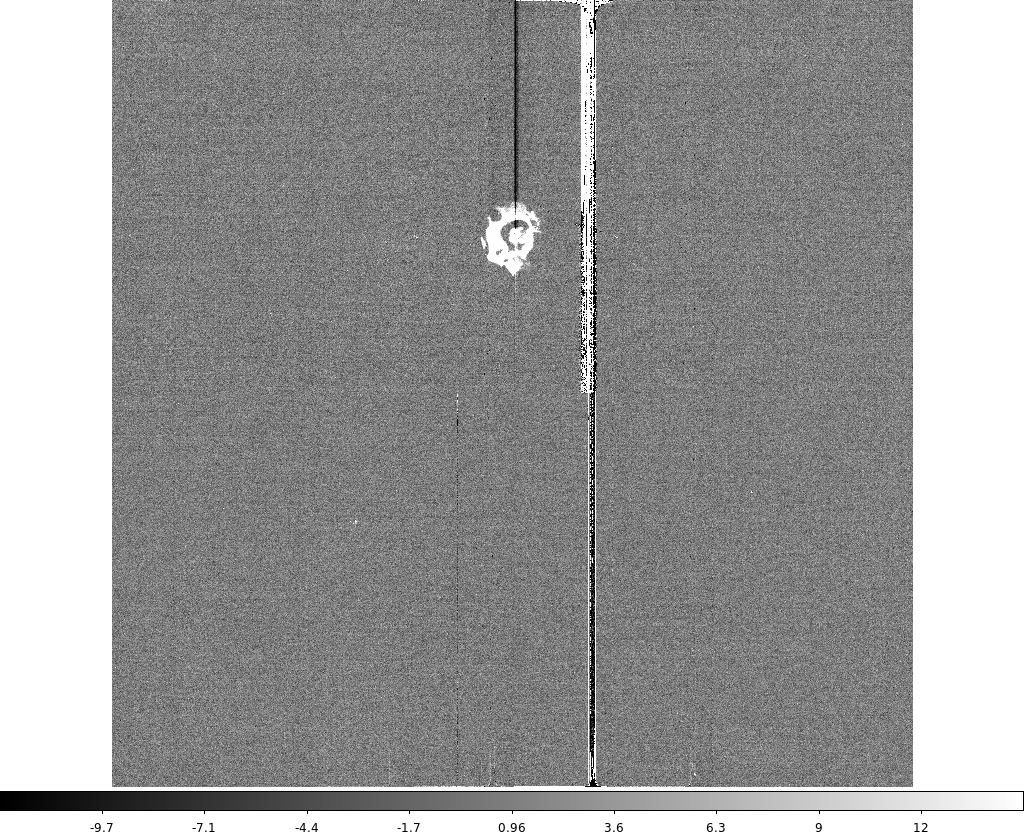
\includegraphics[width=.6\linewidth]{sections/figures/phosphorescence-survey/stains_phos_R01_S00.png}    
\end{minipage}
\begin{minipage}{1.0\textwidth}
  \centering
  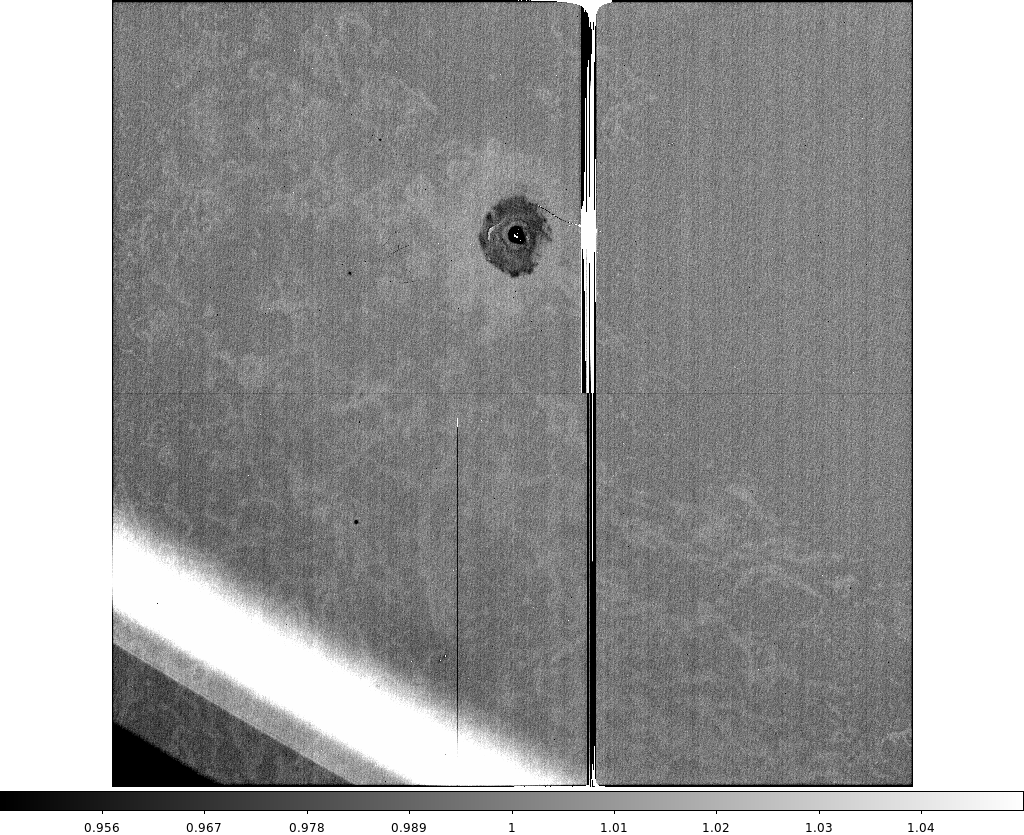
\includegraphics[width=.6\linewidth]{sections/figures/phosphorescence-survey/stains_abs_R01_S00.png}
\end{minipage}
\caption{The ITL sensor R01\_S00. Top: the transient phosphorescence term. Bottom: the {\it blue} flat response. The large, extended spot appears to be centered on a {\it vampire pixel}, which also expresses a large amplitude of phosphorescence, which emits enough current to contaminate the parallel overscan in at least the first 15\,s exposure following trigger. The flat response feature has opposite polarity from the phosphorescence.}
\label{fig:phos:stains:R01S00}
\end{figure}


\begin{figure}[!htbp]
\centering
\begin{minipage}{1.0\textwidth}    
  \centering
  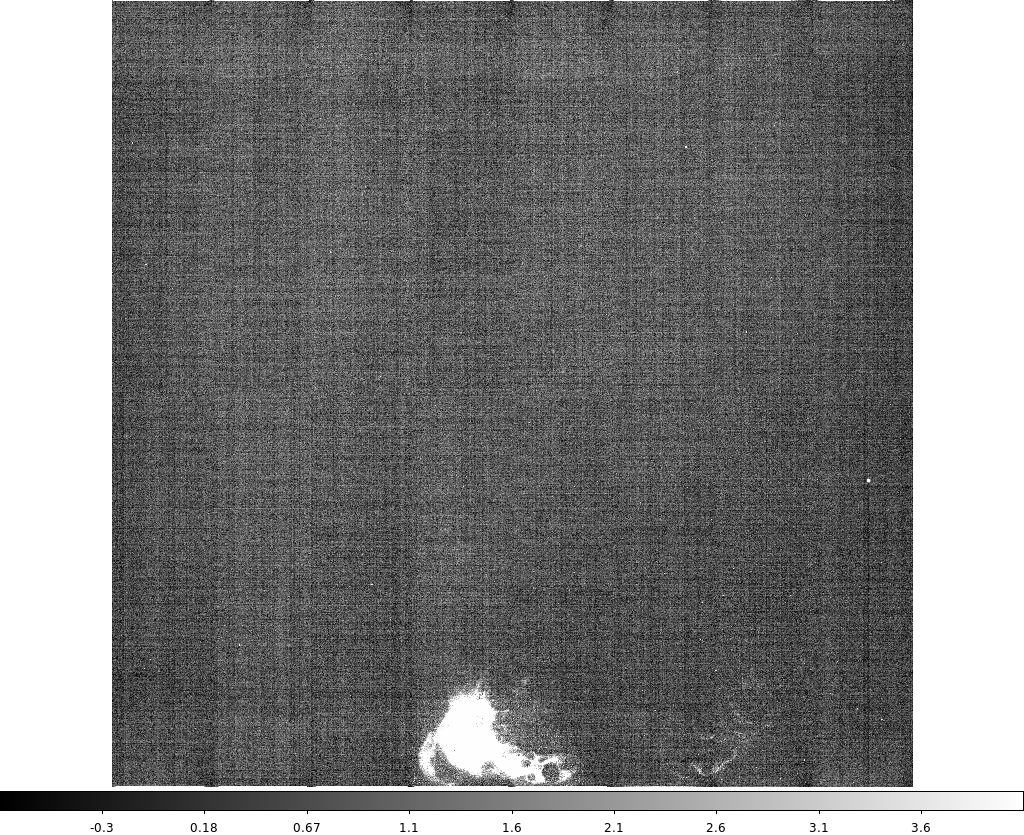
\includegraphics[width=.6\linewidth]{sections/figures/phosphorescence-survey/stains_phos_R02_S02.png}    
\end{minipage}
\begin{minipage}{1.0\textwidth}
  \centering
  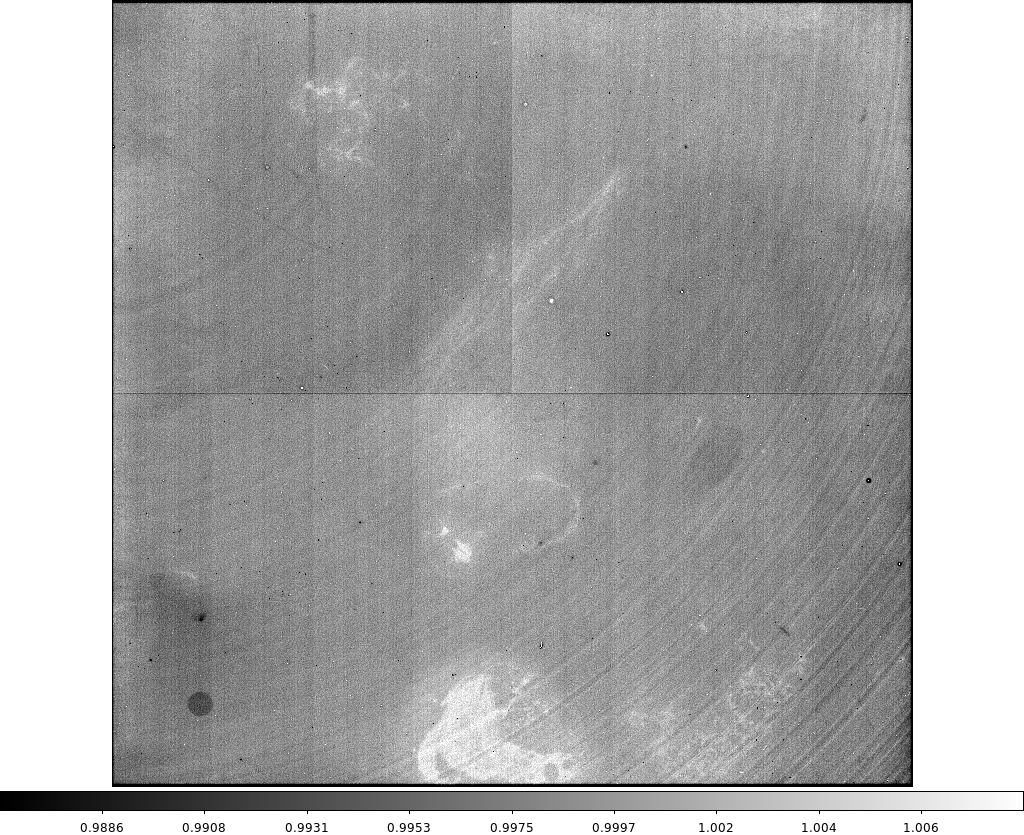
\includegraphics[width=.6\linewidth]{sections/figures/phosphorescence-survey/stains_abs_R02_S02.png}
\end{minipage}
\caption{The ITL sensor R02\_S02. Top: the transient phosphorescence term. Bottom: the {\it blue} flat response. The {\it coffee stain} feature in the flat response has the same polarity as the phosphorescence. A phosphorescent {\it vampire pixel} is seen in segment R02\_S02\_C07.}
\label{fig:phos:stains:R02S02}
\end{figure}

\begin{figure}[!htbp]
\centering
\begin{minipage}{1.0\textwidth}    
  \centering
  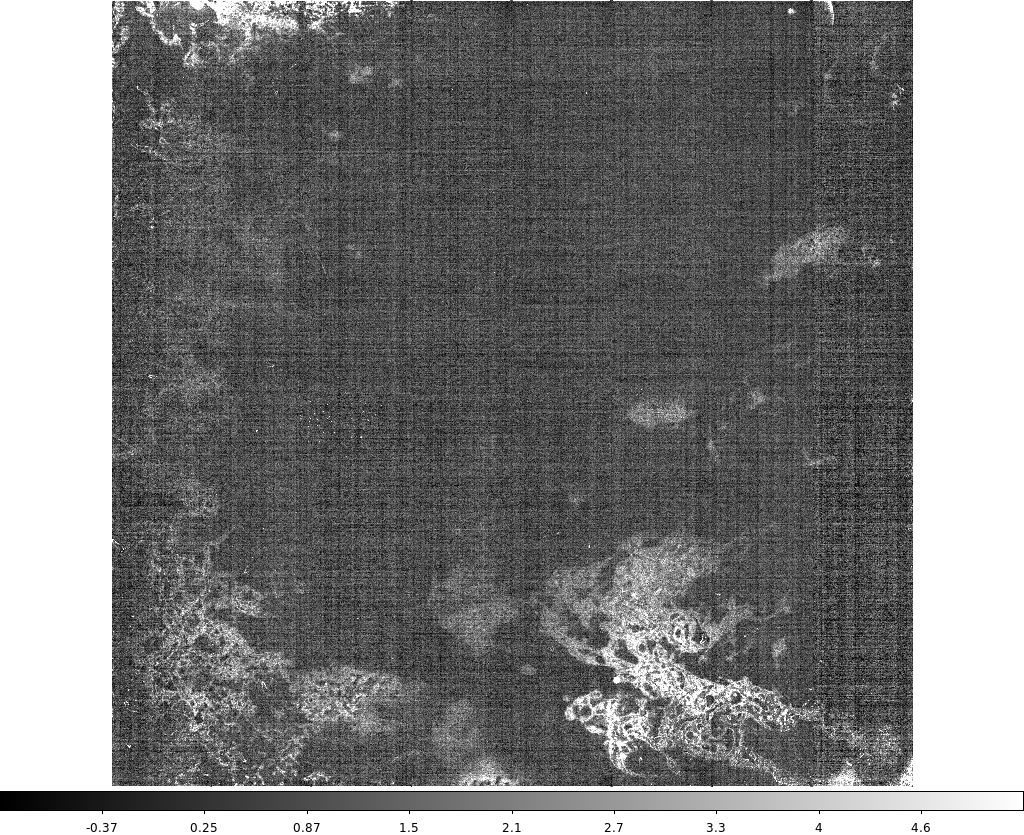
\includegraphics[width=.6\linewidth]{sections/figures/phosphorescence-survey/stains_phos_R02_S12.png}    
\end{minipage}
\begin{minipage}{1.0\textwidth}
  \centering
  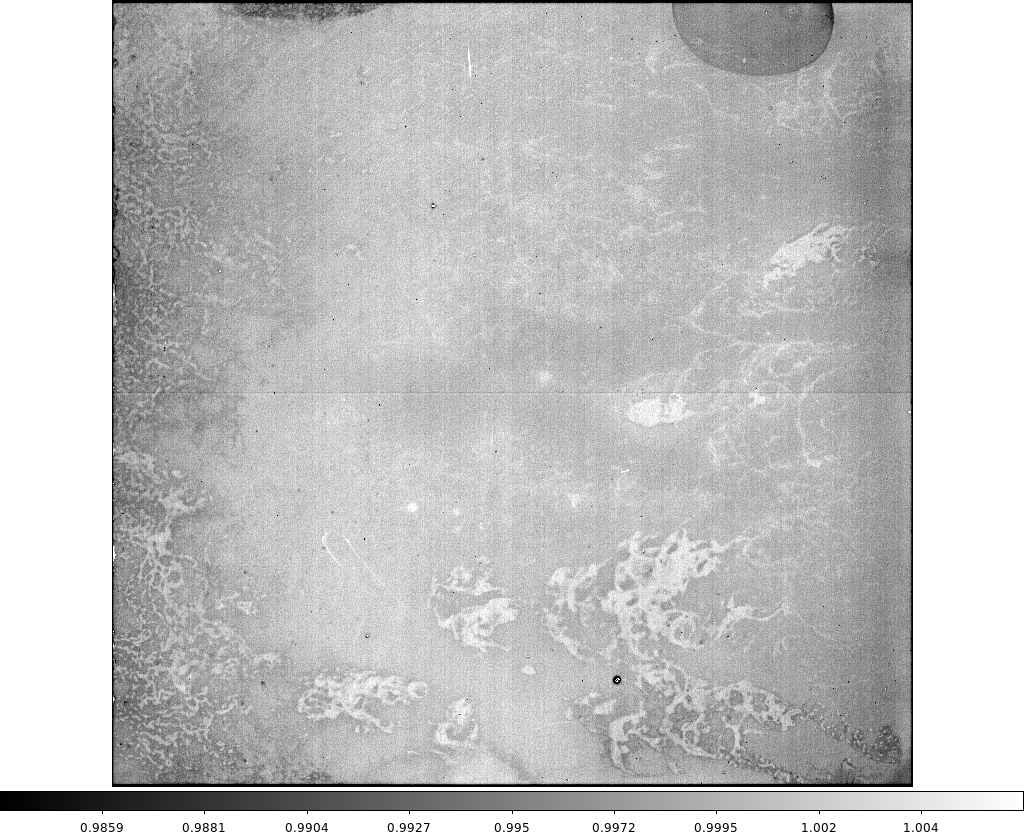
\includegraphics[width=.6\linewidth]{sections/figures/phosphorescence-survey/stains_abs_R02_S12.png}
\end{minipage}
\caption{The ITL sensor R02\_S12. Top: the transient phosphorescence term. Bottom: the {\it blue} flat response. Generally the polarity of the phosphorescence matches that of the {\it coffee stain} in the flat field response, but exceptions include the {\it vampire pixel} seen in segment R02\_S12\_C05.}
\label{fig:phos:stains:R02S12}
\end{figure}


\begin{figure}[!htbp]
\centering
\begin{minipage}{1.0\textwidth}    
  \centering
  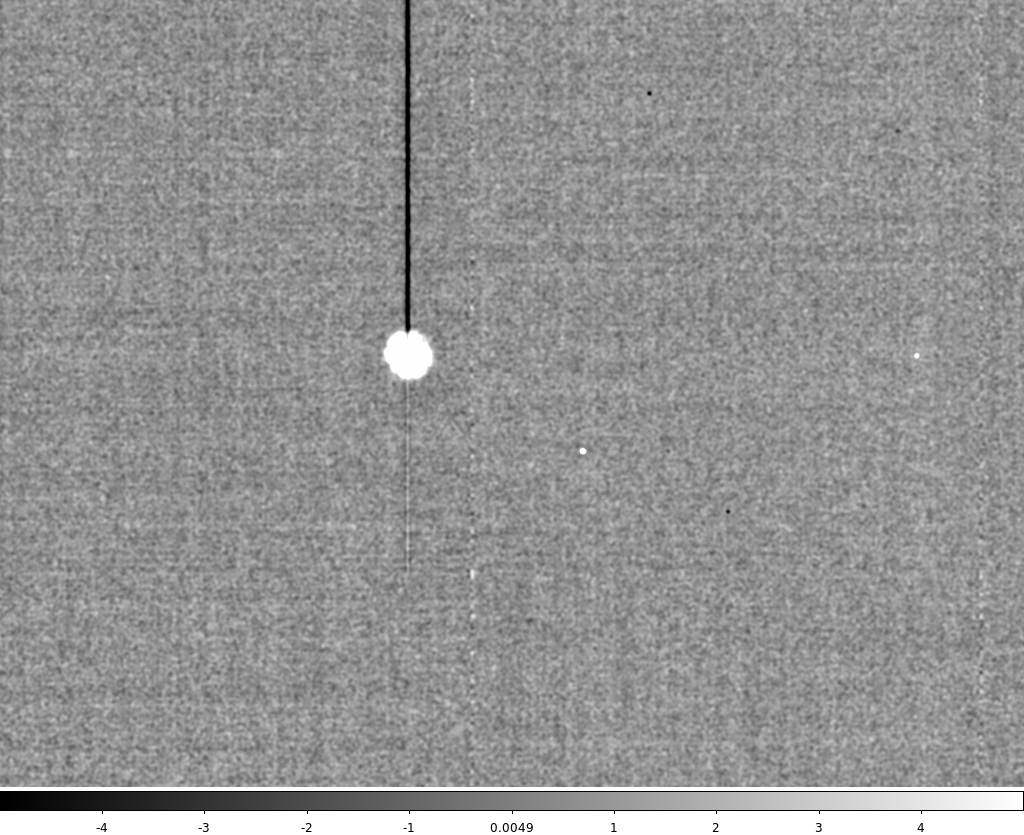
\includegraphics[width=.6\linewidth]{sections/figures/phosphorescence-survey/stains_phos_R03_S10.png}    
\end{minipage}
\begin{minipage}{1.0\textwidth}
  \centering
  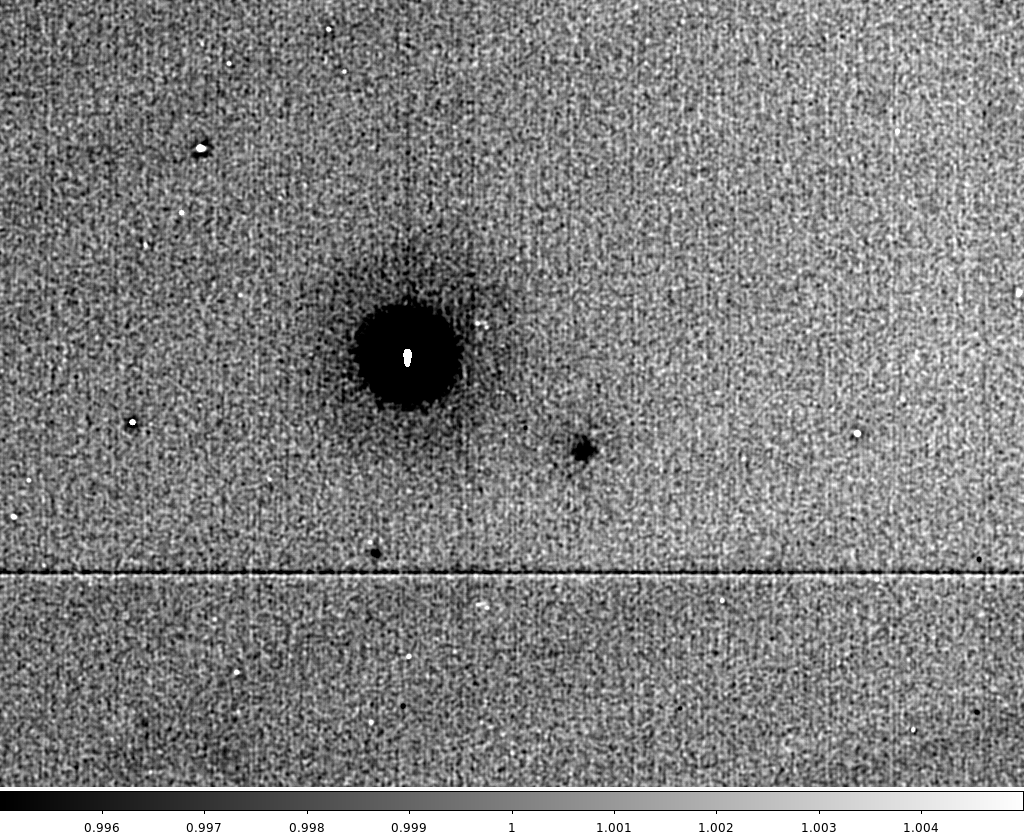
\includegraphics[width=.6\linewidth]{sections/figures/phosphorescence-survey/stains_abs_R03_S10.png}
\end{minipage}
\caption{The ITL sensor R03\_S10, detail of the {\it vampire pixel} of R03\_S10\_C15. Top: the transient phosphorescence term. Bottom: the {\it blue} flat response. As in previous examples, this {\it vampire pixel}'s transient term is large enough to contaminate the parallel overscan even after the first 15\,s following trigger.}
\label{fig:phos:stains:R03S10}
\end{figure}


\begin{figure}[!htbp]
\centering
\begin{minipage}{1.0\textwidth}    
  \centering
  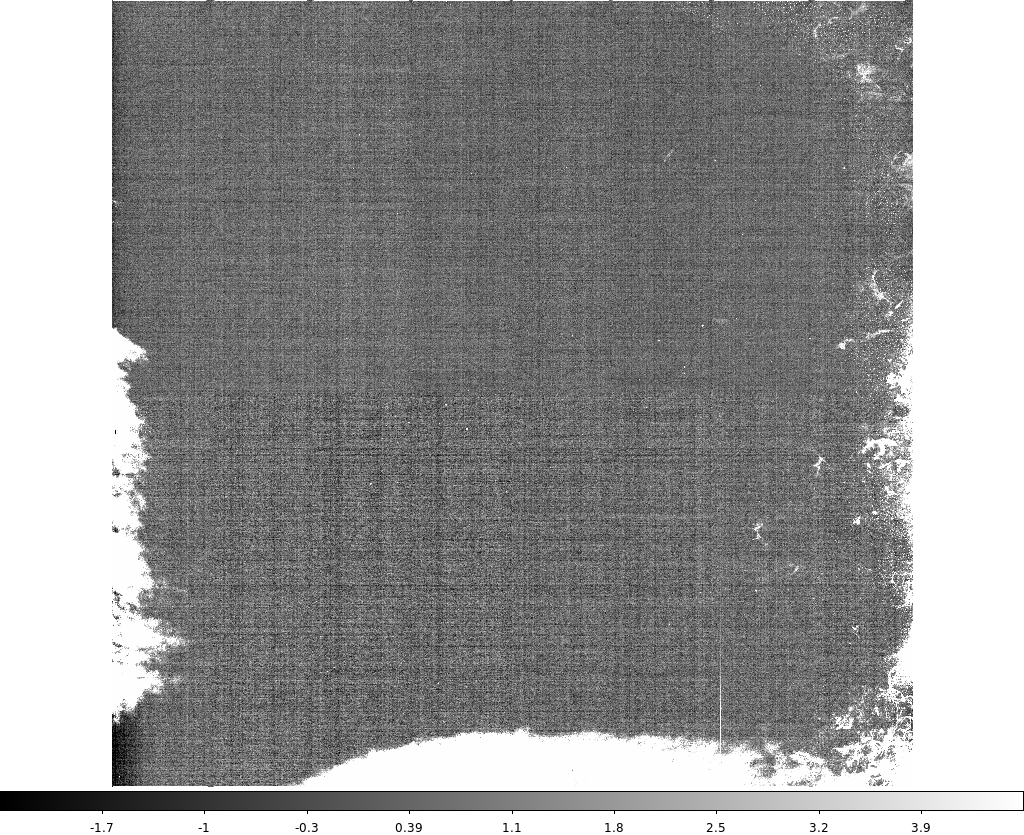
\includegraphics[width=.6\linewidth]{sections/figures/phosphorescence-survey/stains_phos_R43_S11.png}    
\end{minipage}
\begin{minipage}{1.0\textwidth}
  \centering
  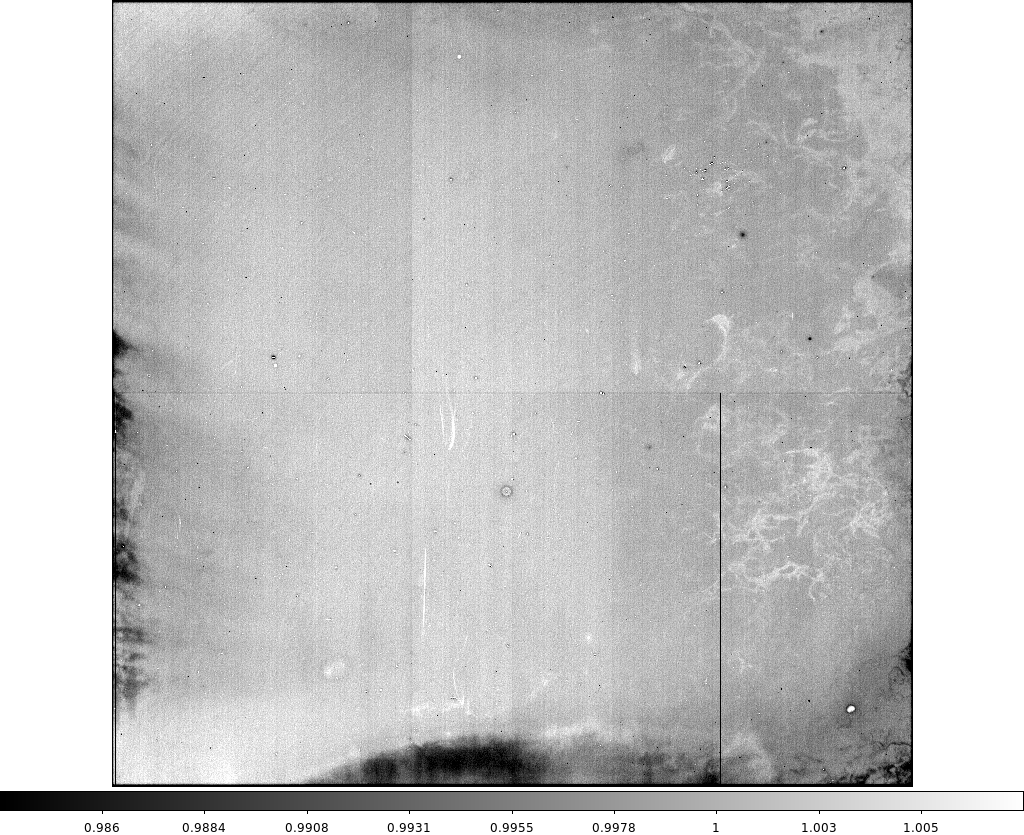
\includegraphics[width=.6\linewidth]{sections/figures/phosphorescence-survey/stains_abs_R43_S11.png}
\end{minipage}
\caption{The ITL sensor R43\_S11. Top: the transient phosphorescence term. Bottom: the {\it blue} flat response. This sensor appears to have the largest integrated phosphorescence among ITL sensors studied. The flat response feature has opposite polarity from the phosphorescence.}
\label{fig:phos:stains:R43S11}
\end{figure}


\begin{figure}[!htbp]
\centering
\begin{minipage}{1.0\textwidth}    
  \centering
  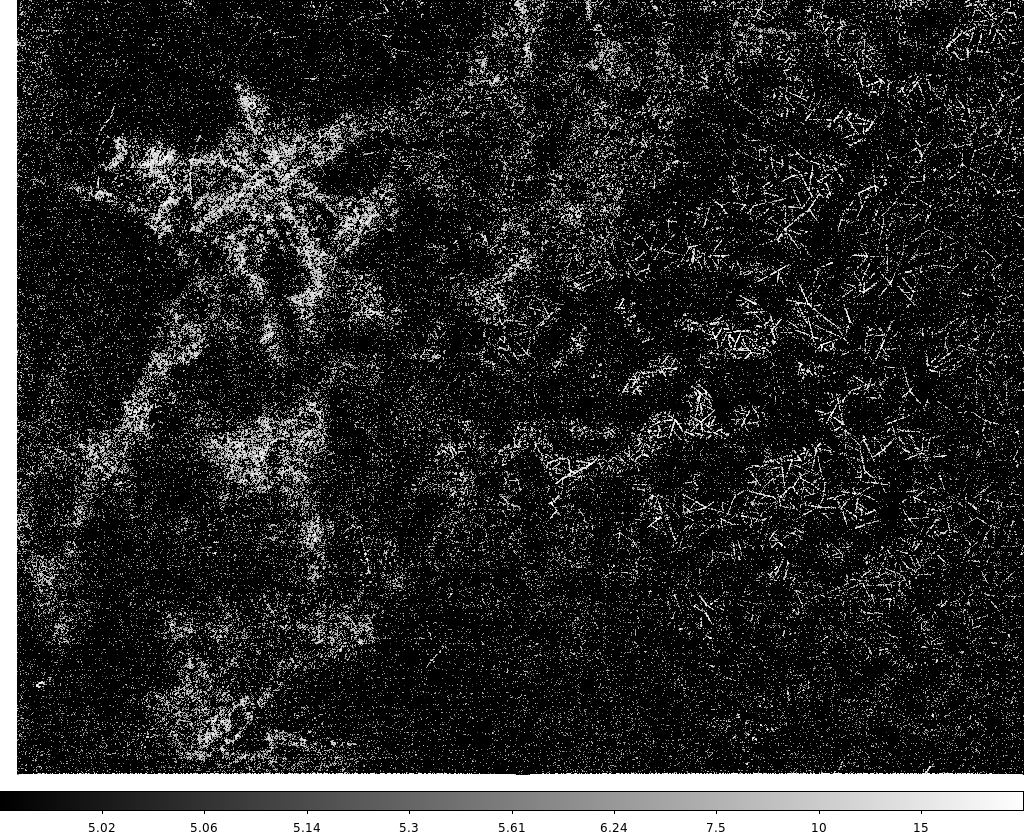
\includegraphics[width=.6\linewidth]{sections/figures/phosphorescence-survey/stains_phos_R43_S20_detail.png}    
\end{minipage}
\begin{minipage}{1.0\textwidth}
  \centering
  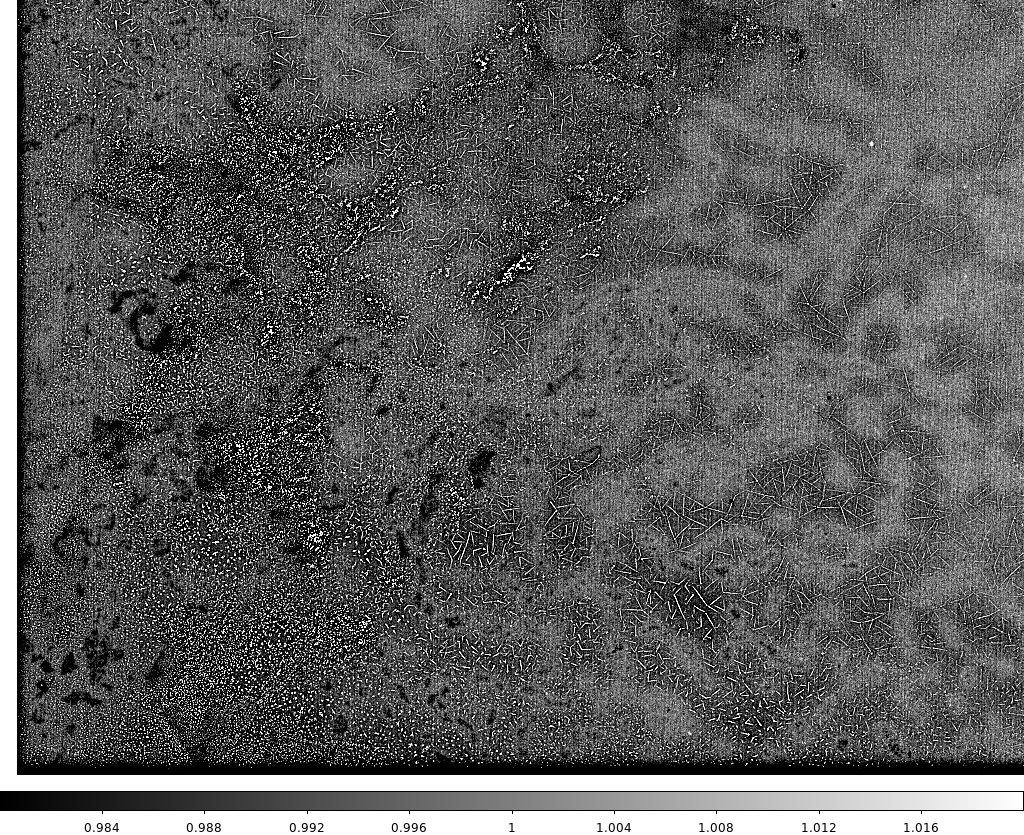
\includegraphics[width=.6\linewidth]{sections/figures/phosphorescence-survey/stains_abs_R43_S20_detail.png}
\end{minipage}
\caption{The ITL sensor R43\_S20, segments C00 through C03. Top: the transient phosphorescence term. Bottom: the {\it blue} flat response. This sensor apparently exhibits peculiar radial crazing patterns seen in both phosphorescence as well as in flat field response, with polarities aligned.}
\label{fig:phos:stains:R43S20}
\end{figure}
